\chapter{Minimum Spanning Trees}
\newcommand{\boruvka}{Bor\r{u}vka\xspace}
\label{ch:mst}

\begin{notesonly}

Concepts:

\begin{itemize}

\item Puzzle 1: you have 6 cities as shown in the example and you can
  build roads between some of these cities as shown. Your task is to
  connect all cities by building the smallest number of road segments.
  How many edges you need?  5 because all you need is a tree.

\item Puzzle 2: suppose now you have edge weights.  you want to build
  the spanning tree that has the minumum total weight.
\end{itemize}


Algorithms for Spanning trees.
\begin{itemize}

\item BFS, DFS


\item Graph contraction based algorithm. Select star edges as tree edges.

\item Iterative algorithm: add each edge one by one unless the
  endpoints are in the same component.  Excellent way to introduce
  union find. TODO: Show how to implement union find on log work/span.

\end{itemize}



Algorithms for  Minimum Spanning Trees
\begin{itemize}

\item Introduce light edge rule by considering a cut consisting of a
  single vertex.  The lightest edge on that vertex v must be in the
  MST.  Suppose not.  Consider adding the lightest edge.  There is a
  cycle, because there is an edge from (u1, v) and the lightest edge
  (u2,v).  Replace (u1,v) with (u2,v).  You have  a tree with smaller
  weight.

\item Go back to your example and check that this is the case.

\item Now generalize.  the point is that you can consider any cut and
  replace the heaving edge crossing the cut with the lightest. You
  still have a spanning tree because when you delete the heavy edge.
  you get two trees, which then you connect by inserting the lightest
  edge. 


\item Now go trough, Prim, Kruskal, and Boruvka.


\item For Boruvka: establish that each part is a tree.  By arguing why
  you can't have cycles. A cycle would violate the ordering relation
  assumed for picking joiners.

\end{itemize}



\end{notesonly}

In this chapter we cover a important graph problem, Minimum Spanning
Trees (MST).  The MST of an undirected, weighted graph is a tree that
spans the graph while minimizing the total weight of the edges in the
tree.  We first define spanning tree and minimum spanning trees
precisely and then present two sequential algorithm and one parallel
algorithm, which are respectively Kruskal's, Prim's, and \boruvka's.
All of these algorithms utilize an important cut property, which we
also desribe.

\ur{2013: The arguments for correctness and complexity needs to be improved.}

\section{Minimum Spanning Trees}
\label{sec:mst::mst}
Recall that we say that an undirected graph is a forest if it has no
cycles and a tree if it is also connected. Given a connected,
undirected graph, we might want to identify a subset of the edges that
form a tree, while ``touching'' all the vertices.  We call such a tree
a spanning tree.
%
\begin{definition}
For a connected undirected graph $G = (V,E)$, a spanning tree is a
tree $T = (V,E')$ with $E' \subseteq E$.
\end{definition}
Note that a graph can have many spanning trees, but all have $|V|$
vertices and $|V|-1$ edges.

\begin{example}
A graph on the left, and two possible spanning trees.
\begin{center}
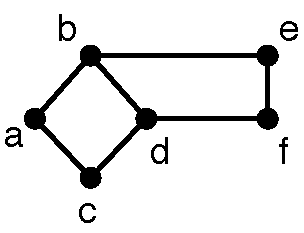
\includegraphics[width=1.7in]{min-spanning-tree/graph-pistol}
\hspace{.1in}
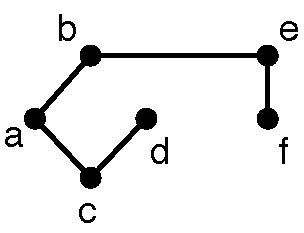
\includegraphics[width=1.7in]{min-spanning-tree/graph-pistol-st-1}
\hspace{.1in}
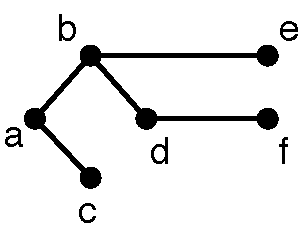
\includegraphics[width=1.7in]{min-spanning-tree/graph-pistol-st-2}
\end{center}
\end{example}


\begin{question}
Design an algorithm for finding a spanning tree of a connected,
undirected graph?
\end{question}

One way to generate a spanning tree is simply to do a graph search.
For example the DFS-tree of a DFS is a spanning tree, as it finds a
path from a source to all the vertices. Similarly, we can construct a
spanning tree based on BFS, by adding each edge that leads to the
discovery of an unvisited vertex to the tree.  DFS and BFS are
work-efficient algorithms for computing spanning trees but as we
discussed they are not good parallel algorithms.
\begin{question}
Can you think of an algorithm with polylogarithmic span for finding a
spanning tree of a connected undirected graph? 
\end{question}
Another way to generate a spanning tree is to use graph contraction,
which as we have seen can be done in parallel.  The idea is to use
star contraction and add all the edges that are selected to define the
stars throughout the algorithm to the spanning tree.

Recall that a graph has many spanning trees.  In weighted graphs, we
may be interested in finding the spanning tree with the smallest total
weight (i.e. sum of the weights of its edges).

\begin{definition}
Given a connected, undirected weighted graph $G = (V,E,w)$, the
minimum (weight) spanning tree (MST) problem requires finding a
spanning tree of minimum weight, where the weight of a tree $T$ is
defined as:
\[
w(T) = \sum_{e \in E(T)} w(e).
\]
\end{definition}

\begin{example}
A graph (left) and its MST (right). 
\begin{center}
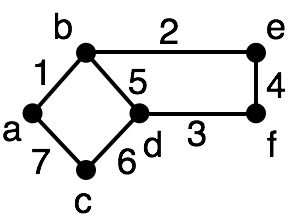
\includegraphics[width=2in]{min-spanning-tree/graph-pistol-w}
%graph-pistol-w-cut-1.pdf 
%
\hspace{1in}
%
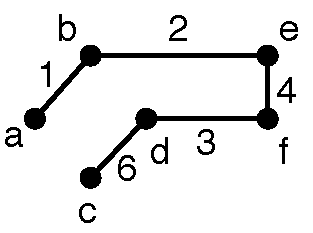
\includegraphics[width=2in]{min-spanning-tree/graph-pistol-w-mst}
\end{center}
\end{example}



\begin{example}
\label{ex:mst::network-design}
Minimum spanning trees have many interesting applications. One example
concerns the design of a network.  Suppose that you are wiring a
building so that all the rooms are connected via bidirectional
communication wires.  Suppose that you can connect any two rooms at
the cost of the wire connecting the rooms, which depends on the
specifics of the building and the rooms but is always a positive real
number.  We can represent the possible connection between rooms as a
graph, where vertices represent rooms and weighted edges represent
possible connections along with their cost (weight).  To minimize the
cost of the wiring, you could find a minimum spanning tree of the
graph.  

\end{example}

\section{Algorithms for Minimum Spanning Trees}

There are several algorithms for computing minimum spanning trees.
They all, however, are based on the same underlying property about
cuts in a graph, which we will refer to as the \defn{light-edge
  property}.  Intuitively, the light-edge property (precisely defined
below) states that if you partition the graph into two, the minimum
edge between the two parts has to be in the MST.  The light-edge
property gives a way to identify algorithmically the edges of an MST.
%

In our discussion we will assume that all edges have distinct
weights. This assumption causes no loss-of-generality, because
light-edge property allows us to break ties arbitrarily, which we can
take advantage of by for example breaking ties based on some arbitrary
ordering of edges such as their position in the input.
%
\begin{question}
Consider a graph where each edge has a distinct weight, how many MST's
can the graph have?
\end{question}
%
A simplifying consequence of this assumption is that the MST of a
graph with distinct edge weights is unique.


\begin{definition}[Graph Cut]
For a graph $G = (V,E)$, a cut is defined in terms of a
non-empty proper subset $U \subsetneq V$.  The set $U$ partitions the
graph into $(U, V \setminus U)$, which is called the \defn{cut}.
%
We refer to the edges between the two parts as the \defn{cut edges}
written $E(U,\overline{U})$, where $\overline{U} = V \setminus U$.
\end{definition}

The subset $U$ used in the definition of a cut might include a single
vertex $v$, in which case the cut edges would be all edges incident on
$v$.  But the subset $U$ must be a proper subset of $V$ (i.e., $U \neq
V$).  We sometimes say that a cut edge  \defn{crosses} the cut.

%% Note: the definition above excluded empty set from a proper set
%% A proper set can be empty.


\begin{example}
Two example cuts.  For each cut, we can find the lightest edge that
crosses that cut, which are the edges with weight $2$ (left) and $4$
(right) respectively.
\begin{center}
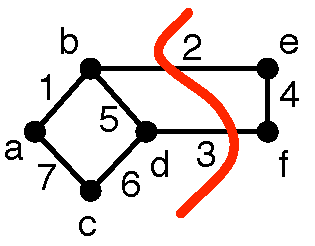
\includegraphics[width=2in]{min-spanning-tree/graph-pistol-w-cut-1}
%graph-pistol-w-cut-1.pdf 
%
\hspace{1in}
%
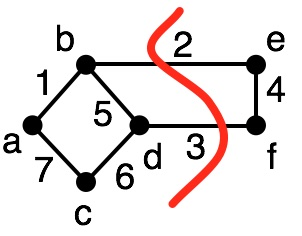
\includegraphics[width=2.4in]{min-spanning-tree/graph-pistol-w-cut-2}
\end{center}
\end{example}



\begin{figure}
\begin{lemma}[Light-Edge Property] 
  Let $G = (V,E,w)$ be a connected undirected weighted graph with
  distinct edge weights.  For any cut of $G$, the minimum weight edge
  that crosses the cut is in the minimum spanning tree MST($G$) of
  $G$.
\label{lem:mst::cut}


\begin{center}
  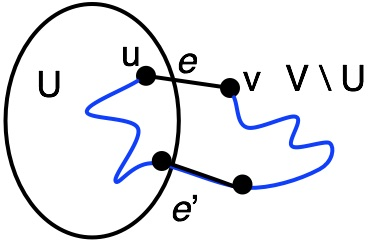
\includegraphics[width=2.2in]{min-spanning-tree/red-blue-fig1}
\end{center}

\begin{proof}
  The proof is by contradiction.  Assume the minimum-weighted edge $e
  = (u,v)$ is not in the MST.  Since the MST spans the graph, there
  must be some simple path $P$ connecting $u$ and $v$ in the MST
  (i.e., consisting of just edges in the MST).  The path must cross
  the cut between $U$ and $V\setminus U$ at least once since $u$ and
  $v$ are on opposite sides. Let $e'$ be an edge in $P$ that crosses
  the cut.  By assumption the weight of $e'$ is larger than that of
  $e$.  Now, insert $e$ into the graph---this gives us a cycle
  that includes both $e$ and $e'$---and remove $e'$ from the graph to
  break the only cycle and obtain a spanning tree again.
%This uses the facts that (1)
%  adding an edge to a spanning tree creates a cycle, and (2) removing
%  any edge from this cycle creates a tree again.  
  Now, since the
  weight of $e$ is less than that of $e'$, the resulting spanning tree
  has a smaller weight.  This is a contradiction and thus $e$ must
  have been in the tree.
\end{proof}
\end{lemma}
\end{figure}


An important implication of the light-edge property as proved in
\lemref{mst::cut} is that any minimum-weight edge that crosses a cut
can be immediately added to the MST.  In fact, all of the three
algorithms that we will consider in this chapter take advantage of
this implication.
%
For example, Kruskal's algorithm constructs the MST by greedily adding
the overall minimum edge.  Prim's algorithm grows an MST incrementally
by considering a cut between the current MST and the rest of
graph. \boruvka's algorithm constructs a tree in parallel by
considering the cut defined by each and every vertex.
%
In the next section, we briefly review Kruskal's and Prim's algorithm
and spend most of our time on a parallel variant of \boruvka's
algorithm.



\begin{remark}
Even though \boruvka's algorithm is not the only parallel algorithm, it
was the earliest, invented in 1926, as a method for constructing an
efficient electricity network in Moravia in the Czech Republic.  It
was re-invented many times over.
\end{remark}



\subsection{Kruskal's Algorithm}
As described in Kruskal's original paper, the algorithm is:
\begin{quote}
``Perform the following step as many times as possible: Among the edges
of $G$ not yet chosen, choose the shortest edge which does not form
any loops with those edges already chosen.'' [Kruskal, 1956]
\end{quote}
In more modern terminology we would replace ``shortest'' with
``lightest'' and ``loops'' with ``cycles''.  

Kruskal's algorithm is correct since it maintains the invariant on
each step that the edges chosen so far are in the MST of $G$.  This is
true at the start.  Now on each step, any edge that forms a cycle with
the already chosen edges cannot be in the MST.  This is because adding
it would violate the tree property of an MST and we know, by the
invariant, that all the other edges on the cycle are in the MST.  Now
considering the edges that do not form a cycle, the minimum weight
edge must be a ``light edge'' since it is the least weight edge that
connects the connected subgraph at either endpoint to the rest of the
graph.  Finally we have to argue that all the MST edges have been
added.  Well we considered all edges, and only tossed the ones that we
could prove were not in the MST (i.e. formed cycles with MST edges).

We could finish our discussion of Kruskal's algorithm here, but a few
words on how to implement the idea efficiently are warranted.  In
particular checking if an edge forms a cycle might be expensive if we
are not careful.  Indeed it was not until many years after Kruskal's
original paper that an efficient approach to the algorithm was
developed.  Note that to check if an edge $(u,v)$ forms a cycle, all
one needs to do is test if $u$ and $v$ are in the same connected
component as defined by the edges already chosen.  One way to do
this is by contracting an edge $(u,v)$ whenever it is added---i.e.,
collapse the edge and the vertices $u$ and $v$ into a single
super-vertex.  However, if we implement this as described in the last
chapter we would need to update all the other edges incident on $u$
and $v$.  This can be expensive since an edge might need to be updated
many times.  
%Furthermore the contraction can create duplicate edges
%with different weights.  We would need to allow for duplicate edges,
%or remove all but the lightest of them.

To get around these problem it is possible to update the edges lazily.
What we mean by lazily is that edges incident on a contracted vertex
are not updated immediately, but rather later when the edge is
processed.  At that point the edge needs to determine what
supervertices (components) its endpoints are in.  This idea can be
implemented with a \defn{union-find data structure}.  The ADT for a
union-find data structure consists of the following operations on a
union-find structure $U$:

\begin{itemize}
\item  \texttt{insert}$U$ $v$ inserts the vertex
$v$ into $U$,

\item \texttt{union} $U$ $(u,v)$ joins the two elements $u$ and $v$ into
a single super-vertex, 

\item \texttt{find}$U$ $v$ returns the super-vertex in which $v$
  belongs, possibly itself, 

\item \texttt{equals}$u$ $v$ returns true if $u$ and $v$ are the same
  super-vertex.  Now we can simply process the edges in increasing
  order.  This idea gives \algref{mst::kruskal}.
\end{itemize}

\begin{figure}[tb]
\begin{algorithm}[Union-Find Kruskal]~
\begin{lstlisting}
kruskal $(G = (V,E,w))$ =
  let
    $U$ = iterate insert $\emptyset$ $V$  @\cdc{initialize UF}@
    $E'$ = sort $(E,w)$              @\cdc{sort the edges}@
    addEdge $((U,T),~e = (u,v))$ =
      let
        $u'$ = find $(U,u)$
        $v'$ = find $(U,v)$
      in 
        if $(u' = v')$ then 
          $(U,T)$    @\cdc{if $u$ and $v$ are connected, skip}@
        else 
          @\cdch{contract $e$ and add it to $T$}@
          $($union $(U, u',v'),T \cup e$ $)$  

     end
  in
    iterate addEdge $(U,\emptyset)$ $E'$
  end
\end{lstlisting}
\label{alg:mst::kruskal}
\end{algorithm}
\end{figure}

\begin{comment}
The algorithm is correct since it always takes the lightest weight edge
The intuitive reason for its correctness is that it constructs a
spanning tree by considering the edges from the smallest to the
largest weight.  In other words, it is almost a literal application of
the light-edge rule.  We can argue for correctness more carefully via
proof by contradiction. Assume that the result is wrong.  This means
that some lightest edge $e$ for a cut is not in the MST. Consider the
time at which that $e$ was considered by the algorithm.  Since $e$ is
not chosen, its end points are in the same component and thus there is
a path between them that crosses that path. Consider the edge $e'$
that crosses the cut.  Since the algorithm picks edges in sorted
order, the weight of $e'$ is less than that of $e$. But then $e$ is
not the lightest edge crossing the cut; a contradiction.  We therefore
conclude that $e$ is in the MST and thus the result is correct.
\end{comment}

\begin{question}
What is the work and the span of Kruskal's algorithm based on union-find? 
\end{question}

To analyze the work and span of the algorithm we first note that there
is no parallelism, so the span equals the work.  To analyze the work
we can partition it into the work required for sorting the edges and
then the work required to iterate over the edges using union and find.
The sort requires $O(m \log n)$ work.  The union and find operations
can be implemented in $O(\log n)$ work each requiring another $O(m
\log n)$ work since they are called $O(m)$ times.  The overall work is
therefore $O(m \log n)$.  It turns out that the union and find
operations can actually be implemented with less than $O(\log n)$
amortized work, but this does not reduce the overall work since we
still have to sort.

\subsection{Prim's Algorithm}

Prim's algorithm performs a priority-first search to construct the
minimum spanning tree.  The idea is that if we have already visited a
set $X$, then by the light-edge property the minimum weight edge with
one of its endpoint in $X$ and the other in $V \setminus X$ must be in
the MST (it is a minimum cross edge from $X$ to $V \setminus X$).  We
can therefore add it to the MST and include the other endpoint in $X$.
This leads to the following definition of Prim's algorithm:

\begin{algorithm}[Prim's Algorithm]
For a weighted undirected graph $G=(V,E,w)$ and a source $s$, Prim's
algorithm is priority-first search on $G$ starting at an arbitrary $s
\in V$ with $T = \emptyset$, using priority $\displaystyle p(v) =
\min_{x \in X} w(x,v)$ (to be minimized), and setting $T = T \cup
\cset{(u,v)}$ when visiting $v$ where $w(u,v) = p(v)$.
\end{algorithm}

When the algorithm terminates, $T$ is the set of edges in the MST.

\begin{example}
A step of Prim's algorithm.  Since the edge $(\vname{c},\vname{f})$ has minimum weight
across the cut $(X,Y)$, the algorithm will ``visit'' $\vname{f}$ adding
$(\vname{c},\vname{f})$ to $T$ and $\vname{f}$ to $X$.
\begin{center}
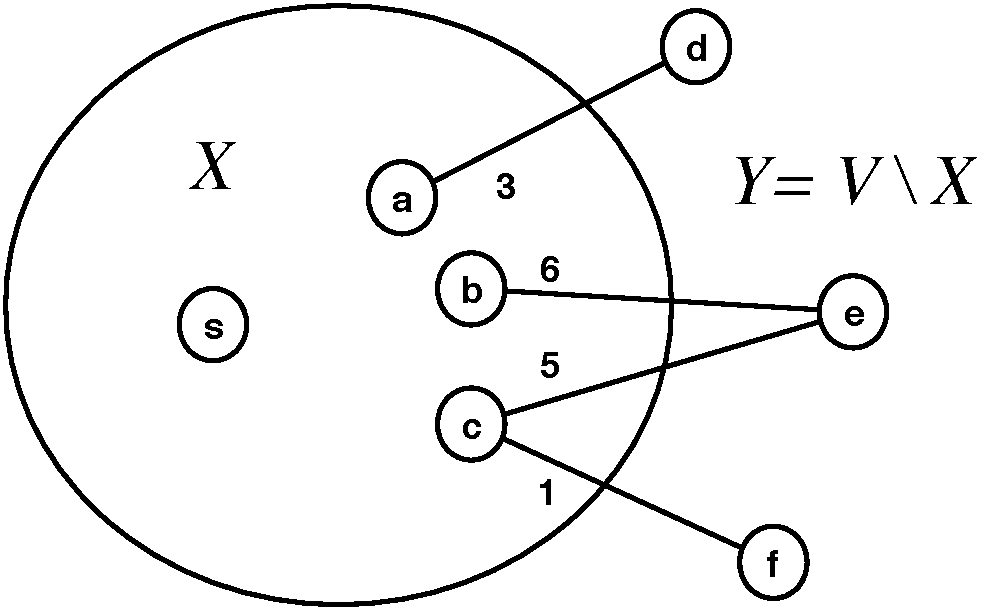
\includegraphics[width=3in]{min-spanning-tree/prims}
\end{center}
\end{example}


\begin{exercise}
Carefully prove the correctness of Prim's algorithm by induction.
\end{exercise}

Interestingly this algorithm is quite similar to Dijkstra's algorithm
for shortest paths.  The only differences are (1) we start at an
arbitrary vertex instead of at a source, (2) that $p(v) = \min_{x \in
  X} (x,v)$ instead of $\min_{x \in X} (d(x) + w(x,v))$, and (3) we
maintain a tree $T$ instead of a table of distances $d(v)$.  Because
of the similarity we can basically use the same priority-queue
implementation as in Dijkstra's algorithm and it runs with the same
$O(m \log n)$ work bounds.


\begin{remark}
  Prim's algorithm was invented in 1930 by Czech mathematician Vojtech
  Jarnik and later independently in 1957 by computer scientist Robert
  Prim.  Edsger Dijkstra's rediscovered it in 1959 in the same paper
  he described his famous shortest path algorithm.
\end{remark}





\begin{comment}
\newcommand{\visitedx}{X}

\begin{pseudocode}[Prim's Algorithm]
\begin{codel}
\cfun~\cname{prim}(G) = \newl
\clet\newl
~~\cfun~\cname{enqueue}~v~(Q,(u, w)) = \cname{PQ.insert}~(w, (v,u))~Q\newlspace{.1in}
~~\cfun~\cname{prim'}(\visitedx,~Q,~T) =\newl
~~~~\ccase~\cname{PQ.deleteMin}(Q)~\cof\newl
~~~~~~~$\=$(\cnone, \cwild) \Rightarrow T~~~~~~~~~~~~~~~~~~~~~~~~\ccomment{Done}\newl
~~~~~|$\>$(\csome(d, (u, v)), Q') \Rightarrow\newl
~~~~~~~\cif~(v \in^? \visitedx)~\cthen~\cname{prim'}(\visitedx,~Q',~T)~~~~~~\cmark\ccomment{Already visited}\newl
~~~~~~~\celse~\clet\newl[line:insert]
~~~~~~~~~\cval~\visitedx' = \visitedx \cup \cset{v}\ctabc{Visit}\newl[line:add]
~~~~~~~~~\cval~T' = T \cup \cset{(u,v)}\ctabc{Add edge to MST}\newl
~~~~~~~~~\cval~Q'' = \citer~(\cname{enqueue}~v)~Q'~N_G(v)\ctabc{Enqueue $v$'s neighbors}\newl
~~~~~~~\cin~\cname{prim'}(\visitedx',~Q'',~T')~\cend\newlspace{.1in}
~~\cval~s = \ctext{an arbitrary vertex from $G$}\newl
~~\cval~Q = \citera{(\cname{enqueue}~s)}{\cset{}}{N_G(s)}\ctabc{Enqueue $s$'s neighbors}\newl
\cin\newl
~~\cname{prim'}(\cset{s},~Q,~\cset{})\newl
\cend
\end{codel}
\end{pseudocode}
\end{comment}


\subsection{\boruvka's Algorithm}


As discussed in previous sections, Kruskal and Prim's algorithm are
sequential algorithms. In this section, we present an MST algorithm
that runs efficiently in parallel using graph contraction.  This
parallel algorithm is based on an approach by \boruvka.  As Kruskal's
and Prim's, \boruvka's algorithm constructs the MST by inserting light
edges but unlike them, it inserts many light edges at once.

To see how we can select multiple light edges, recall that all light
edges that cross a cut must be in the MST.
%
\begin{question}
What is the most trivial cut you can think of?  What edges cross it?
\end{question}
%
Consider now a cut that is defined by a vertex $v$ and the rest of the
vertices in the graph.  
%
The edges that cross this cut are exactly the edges incident on $v$.
%
Therefore, by the light edge rule, for $v$, the minimum weight edge
between it and its neighbors is in the MST.
%
Since this argument applies to all vertices at the same time, the
minimum weight edges incident an any vertex is in the MST.  We call
such edges {\em vertex-joiners}.

\begin{example}
  The vertex-joiners of the graph are highlighted.  
\begin{center}
 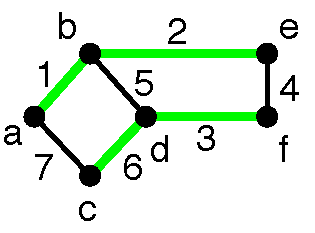
\includegraphics[width=2in]{min-spanning-tree/graph-pistol-w-min}
\end{center}
\end{example}

Since we know that the vertex-joiners are all in the MST, we can
insert them into it in parallel by letting each vertex pick its
vertex-joiner.
%
In the example above, the vertices $\vname{a}$ and $\vname{b}$ both
pick edge $\cset{\vname{a},\vname{b}}$, 
%
vertex $\vname{c}$ picks $\cset{\vname{c},\vname{d}}$, $\vname{d}$,
%
vertex $\vname{f}$ picks $\cset{\vname{d},\vname{f}}$, 
%
and $\vname{e}$ picks $\cset{\vname{e},\vname{b}}$.

\begin{question}
Have we found all the MST edges?  Can we stop? 
\end{question}
Sometimes just one round of picking vertex-joiners will select all the
MST edges and would generate a complete solution.  
%
In most cases, however, the minimum-weight edges on their own do not
form a spanning tree.  
%
In the example above, the edge
$(\vname{e},\vname{f})$, which is in the MST, is not selected (neither
$\vname{e}$ nor $\vname{f}$ pick it).
\begin{question}
Given that we have found some of the edges, how can we proceed, can we
eliminate some edges from consideration?
\end{question}
To see how we can proceed, note that the vertex-joiners define a
partition of the graph---all the vertices are in a part.
%
Consider now the edges that remain internal to a partition but are not
vertex joiners.  
%
Such an edge cannot be in the MST, because inserting it into the MST
would create a cycle.
%
The edges that cross the partitions, however, must be considered as
they can indeed be in the MST.
%

\begin{question}
How can we eliminate the internal edges?
\end{question}
One way to eliminate the internal edges from consideration, while
keeping the cross edges is to perform a graph contraction based on the
partitioning defined by the vertex-joiners. Recall that in graph
contraction, all we need is a partitioning of the graph into disjoint
connected subgraphs.  Given such a partitioning, we then replace each
subgraph (partition) with a super-vertex and relabel the edges.  This
is repeated until no edges remain.
\begin{example}
      Contraction along the minimum edges.   Note that there are
      redundant edges between the two partitions.
\begin{center}
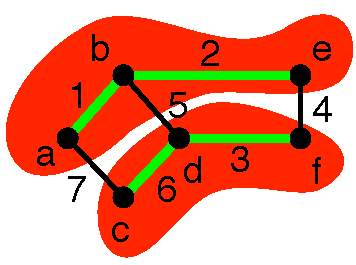
\includegraphics[width=2in]{min-spanning-tree/graph-pistol-w-min-contract}
\hspace{1in}
\raisebox{.5in}{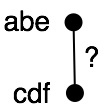
\includegraphics[width=.7in]{min-spanning-tree/graph-pistol-w-contracted}}
\end{center}
\end{example}

When performing graph contraction, we have to be careful about
redundant edges. In our discussion of graph contraction in \chref{gc},
used unweighted graphs, we mentioned that we may treat redundant edges
differently based on the application.  
%
In unweighted graphs, the task is usually simple because we can keep
any one of the redundant edges, and it usually does not matter which
one.  
%
When the edges have weights, however, we have to decide to keep
all the edges or select some of the edges to keep.
\begin{question}
Which edge should we keep for computing the MST?  
\end{question}
%
For the purposes of MST, in particular, we can keep all the edges or
keep just the edge with the minimum weight, because the others, cannot
be in the MST.  In the example above, we would keep the edge with
weight $4$.

What we just covered is exactly \boruvka's idea.  He did not discuss
implementing the contraction in parallel.  At the time, there were not
any computers let alone parallel ones.  We are glad that he has left
us something to do.  In summary, \boruvka's algorithm can be described
as follows.

\begin{algorithm}[\boruvka]
While there are edges remaining: (1) select the minimum weight edge
out of each vertex and contract each part defined by these edges into
a vertex; (2) remove self edges, and when there are redundant edges
keep the minimum weight edge; and (3) add all selected edges to the
MST.
\end{algorithm}

\paragraph{Cost of \boruvka by using tree contraction.}
We now consider the efficiency of this algorithm.  We first focus
on the number of rounds of contraction and
then consider how to implement the contraction.
%
\begin{question}
Suppose that we picked $k$ vertex-joiners, how many vertices
will we remove?
\end{question}
%
Since contracting an edge removes exactly one vertex (contraction of
and edge can be viewed as folding one endpoint into the other), if $k$
edges are selected then $k$ vertices are removed. 
%
\begin{question}
Can we then remove all the vertices? 
\end{question}
%
Since each vertex picks a vertex joiner independently in parallel, it
is possible that $k=n$.
%
In this case, we would be able to fold all the vertices in one round.
%
In the general case, however, one edge can be chosen by two vertices
as vertex joiners.
%
\begin{question}
At least how many vertices can be remove?  
\end{question}
%
Therefore at least $n/2$ vertex joiners are picked and thus $n/2$
vertices will be removed.
%
Consequently, \boruvka's algorithm will take at most $\log_2 n$ rounds
of selecting vertex-joiners and contracting based on the partitioning
defined by them.

\begin{question}
  How can be perform a round of contraction based on the partitioning
  defined by the vertex-joiners? Can we use edge contraction or star
  contraction?
\end{question}
%
To contract the partition defined by the vertex-joiners, we cannot use
edge or star contraction, because the parts may not correspond to an
edge or a star.  
%
% In general each part identified by selecting the
% vertex-joiners are neither single edges nor single stars.
%
\begin{example}
  An example where minimum-weight edges give a non-star tree.  Note
  that we have in fact picked a minimum spanning tree in one round by
  picking the vertex joiners for each vertex.
\begin{center}
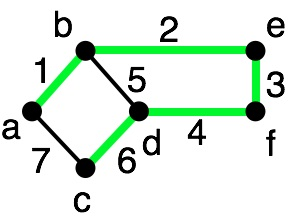
\includegraphics[width=2in]{min-spanning-tree/graph-pistol-w-min-2}
\end{center}
\end{example}
%
It turns out, vertex joiners form a forest (a set of trees).
%
Therefore, each part is a tree and thus we want to contract trees. 
%
By removing all edges that are not vertex-joiners, we can contract a
part by applying star contraction to it.  
%
Furthermore, since when doing a star contraction on a tree, it remains
a tree on each step, the number of edges goes down with the number of
vertices. 
%
Therefore the total work to contract all the partitions is bounded by
$O(n)$ if using array sequences.  The span remains $O(\log^2 n)$.

After contracting each tree, we have to update the edges.  As
discussed earlier for redundant edges we want to keep the minimum
weight such edge.  
%
There are various ways to do this, including keeping the redundant
edges.
%
Keeping the edges turns out to be an effective solution, and allows
the updating the edges to be done in $O(m)$ work.  
%
Assuming redundant edges, the minimum into each component can still be
done with $O(m)$ work, as described below.  Since there are at most
$\log n$ rounds, \boruvka's algorithm will run in $O(m \log n)$ work
and $O(\log^3 n)$ span.

% We now consider how to contract the graph on each round.  This
% requires first identifying the minimum-weight edges.  How this is done
% depends on the graph representation, so we will defer this for the
% moment, and look at the contraction itself once the minimum-weight
% edges have been identified.

\paragraph{Cost of \boruvka by using star contraction.}
We now describe how to improve the span of \boruvka by a logarithmic
factor by interleaving steps of star contraction with steps of finding
the vertex-joiners, instead of fully contracting the trees defined by
the vertex-joiners.  The idea is to apply randomized star contraction
on the subgraph induced by the vertex-joiners, instead of considering
the whole graph as in conventional star contraction.  Intuitively,
this is correct because we only have to care about vertex-joiners (all
other edges cannot be in the MST).
%
As we will show, on each round, we will still be able to reduce the
number of vertices by a constant factor (in expectation), leading to
logarithmic number of total rounds. Consequently, we will reduce the
overall span for finding the MST from $O(\log^3 n)$ to $O(\log^2 n)$
and maintain the same work.

\begin{example}
An example of \boruvka with star contraction. 

\begin{center}
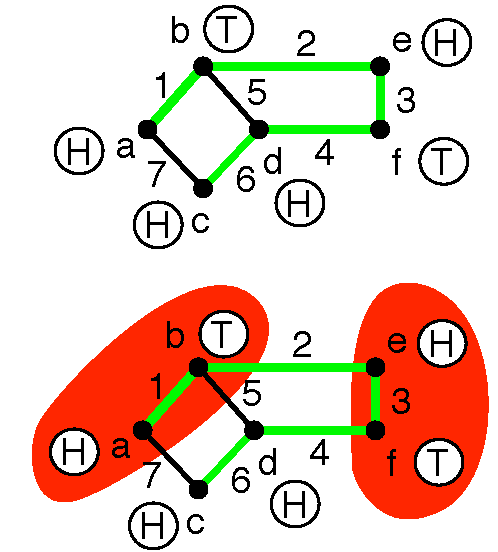
\includegraphics[width=3.25in]{min-spanning-tree/graph-pistol-w-min-2-star-contract}
\end{center}
\end{example}

For a set of vertex-joiners $\mathit{jE}$, consider the subgraph $H =
(V, \mathit{jE})$ of $G$ and apply one step of the star contraction on
$H$.  To apply star contraction, we can modify our
\cname{starContract} routine so that after flipping coins, the tails
only hook across their minimum-weight edge.  \ur{Is there a difference
  between this algorithm and the description above?}  The modified
algorithm for star contraction is as follows.  In the code $w$ stands
for the weight of the edge $(u,v)$.

\begin{algorithm}[Star Contraction along Vertex-Joiners]
~
\begin{lstlisting}
joinerStarContract $(G=(V,E), i)$ =
  let
    jE = vertexJoiners $(G)$
    $P$ = $\csetf{u \mapsto (v,w) \in \cname{jE}}{\neg \cname{heads}(u,i)
    \land \cname{heads}(v,i)}$
    $V'$ = $V \setminus \cname{domain}(P)$
  in 
    $(V',P)$ 
  end
\end{lstlisting}
where $(\cname{vertexJoiners} G)$ finds the vertex-joiners out of each
vertex $v$.
\end{algorithm}

Before we go into details about how we might keep track of the MST and
other information, let us try to understand what effects this change
has on the number of vertices contracted away.  If we have $n$
non-isolated vertices, the following lemma shows that the algorithm
still removes $n/4$ vertices in expectation on each step:

\begin{lemma}
  For a graph $G$ with $n$ non-isolated vertices, let $X_n$ be the random
  variable indicating the number of vertices removed by
  \cname{joinerStarContract}$(G,r)$.  Then, $\expct{X_n} \geq n/4$.
\end{lemma}
\begin{proof}
  The proof is pretty much identical to our proof for
  \cname{starContract} except here we're not working with the whole
  edge set, only a restricted one \cname{jE}.  Let $v \in V(G)$ be a
  non-isolated vertex.  Like before, let $H_v$ be the event that $v$
  comes up heads, $T_v$ that it comes up tails, and $R_v$ that $v \in
  \cname{domain}(P)$ (i.e, it is removed).  Since $v$ is a
  non-isolated vertex, $v$ has neighbors---and one of them has the
  minimum weight, so there exists a vertex $u$ such that $(v,u) \in
  \cname{minE}$.  Then, we have that $T_v \land H_u$ implies $R_v$
  since if $v$ is a tail and $u$ is a head, then $v$ must join $u$.
  Therefore, $\prob{R_v} \geq \prob{T_v} \prob{H_u} = 1/4$.  By the
  linearity of expectation, we have that the number of removed
  vertices is
  \begin{equation*}
    \expct{\sum_{v: v \text{ non-isolated}} \onef{R_v}} = \sum_{v: v \text{ non-isolated}} \expct{\onef{R_v}} \geq n/4
  \end{equation*}
  since we have $n$ vertices that are non-isolated.
\end{proof}

This means that this MST algorithm will take only $O(\log n)$ rounds,
just like our other graph contraction algorithms.

\paragraph{Final Things.} There is a little bit of trickiness since, as the
graph contracts, the endpoints of each edge changes.  Therefore, if we
want to return the edges of the minimum spanning tree, they might not
correspond to the original endpoints.  To deal with this, we associate
a unique label with every edge and return the tree as a set of labels
(i.e. the labels of the edges in the spanning tree).  We also
associate the weight directly with the edge.  The type of each edge is
therefore $(\cname{vertex} \times \cname{vertex} \times \cname{weight}
\times \cname{label})$, where the two vertex endpoints can change as
the graph contracts but the weight and label stays fixed.  This leads
to the slightly-updated version of \cname{joinerStarContract} that
appears in \algref{mst::starBoruvka}.

\begin{figure}
\begin{algorithm}[\boruvka's based on Star Contraction]~
\label{alg:mst::starBoruvka}
\begin{lstlisting}
vertexJoiners $E$ =
  let
    $ET$ = $\cset{(u,v,w,l)\mapsto\cset{u\mapsto(v,w,l)} : (u,v,w,l) \in E}$
    joinEdges $((v_1,w_1,l_1),(v_2,w_2,l_2)) =$
      if $(w_1 \leq w_2)$ then $(v_1,w_1,l_1)$ else $(v_2,w_2,l_2)$ 
  in 
    reduce (union joinEdges) $\cset{}$ $ET$
  end 
@\vspace{.15in}@
joinerStarContract $(G=(V,E), i)$
  let
    $\mathit{minE}$ = vertexJoiners $G$          @\label{line:mst::minedges}@
    $P =\csetf{(u \mapsto (v,w,\ell)) \in \mathit{minE}}{\neg \cname{heads}(u,i)
                     \land \cname{heads}(v,i)}$      @\label{line:mst::hooks}@
    $V' = V \setminus \cname{domain}(P)$     @\label{line:mst::newvertices}@
    in 
      $(V',P)$ 
    end
@\vspace{.15in}@
MST $((V,E),T,i) =$
  if $(|E| = 0)$ then $T$
  else 
  let
    $(V',PT) =$ joinerStarContract $((V,E), i)$
    $P = \cset{u \mapsto v : u \mapsto (v,w,\ell) \in PT} \cup
  \cset{v \mapsto v : v \in V'}$
    $T' = \cset{\ell : u \mapsto (v,w,\ell) \in PT}$
    $E' = \csetf{(\cget{P}{u},\cget{P}{v},w,l) : (u,v,w,l) \in E}{\cget{P}{u} \neq \cget{P}{v}}$
  in
    MST $((V',E'),T \cup T',i+1)$
  end
\end{lstlisting}
\end{algorithm}
\end{figure}

The function $\cname{vertexJoiner}(G)$ in \lineref{mst::minedges}
finds the minimum edge out of each vertex $v$ and maps $v$ to the pair
consisting of the neighbor along the edge and the edge label.  By
\lemref{mst::cut}, since all these edges are minimum out of the
vertex, they are safe to add to the MST.  \lineref{mst::hooks} then
picks from these edges the edges that go from a tail to a head, and
therefore generates a mapping from tails to heads along minimum edges,
creating stars.  Finally, \lineref{mst::newvertices} removes all
vertices that are in this mapping to star centers.

This is ready to be used in the MST code, similar to the
\cname{graphContract} code studied last time, except we return the set
of labels for the MST edges instead of the remaining vertices.   The
code is given in \algref{mst::starBoruvka}
The MST algorithm is called by running $\cname{MST}(G, \emptyset, r)$.  As an 
aside, we know that $T$ is a spanning forest on the contracted nodes. 

Finally we describe how to implement \cname{minEdges}$(G)$, which
returns for each vertex the minimum edge incident on that vertex.
There are various ways to do this.  One way is to make a singleton
table for each edge and then merge all the tables with an appropriate
function to resolve collisions.  \algref{mst::starBoruvka} gives
code that merges edges by taking the one with lighter edge weight.

If using sequences for the edges and vertices an even simpler way is
to presort the edges by decreasing weight and then use \cname{inject}.
Recall that when there are collisions at the same location
\cname{inject} will always take the last value, which will be the one
with minimum weight.

\begin{comment}
\section{Maximal Independent Set (MIS)}

In graph theory, an \emph{independent set} is a set of vertices from an
undirected graph that have no edges between them.  More formally, let a graph $G
= (V, E)$ be given. We say that a set $I \subseteq V$ is an independent set if
and only if $(I \times I) \cap E = \emptyset$.

For example, if vertices in a graph represent entities and edges represent
conflicts between them, an independent set is a group of non-conflicting
entities, which is a natural thing to want to know.  This turns out to be an
important substep in several parallel algorithms since it allows one to find
sets of things to do in parallel that don't conflict with each other.  For this
purpose, it is important to select a large independent set since it will allow
more things to run in parallel and presumably reduce the span of the algorithm.

Unfortunately, the problem of finding the overall largest independent
set---known as the Maximum Independent Set problem---is \textbf{NP}-hard. Its
close cousin Maximal Independent Set, however, admits efficient algorithms and
is a useful approximation to the harder problem.

More formally, the \emph{Maximal Independent Set} (MIS) problem is: given
an undirected graph $G = (V,E)$, find an independent set $I \subseteq V$
such that for all $v \in (V\setminus I)$, $I \cup \{v\}$ is not an
independent set. Such a set $I$ is maximal in the sense that we can't add
any other vertex and keep it independent, but it easily may not be a
maximum---i.e. largest---independent set in the graph.

\begin{center}
  \includegraphics[scale=.7]{min-spanning-tree/mis-example1}
\end{center}

For example, in the graph above, the set $\{a, d\}$ is an independent set,
but not maximal because $\{a, d, e\}$ is also an independent set. On the
other hand, the set $\{a, f\}$ is a maximal independent set because there's
no vertex that we can add without losing independence. Note that in MIS, we
are \emph{not} interested in computing the overall-largest independent set:
while maximum independent sets are maximal independent sets, maximal
independent set are not necessarily maximum independent sets!  Staying with
the example above, $\{a,f\}$ is a maximal independent set but not a maximum
independent set because $\{a, d, e\}$ is independent and larger.

\subsection{Sequential MIS}

Let's first think about how we would compute an MIS if we don't care about
parallelism. We will start by thinking about the effect of picking a vertex $v$
as part of our independent set $I$. By adding $v$ to $I$, we know that none of
$v$'s neighbors can be added to $I$. This motivates an algorithm that picks an
arbitrary vertex $v$ from $G$, add $v$ to $I$, and derive $G'$ from $G$ such
that each vertex of $G'$ is independent of $I$ and can be picked in the next
step. We have the following algorithm:
\begin{codel}
\cfun~\cname{seqMIS}((V,E), I) =\newl
\cif~|V| = 0~\cthen~I~\celse\newl
~~\clet\newl
~~~~\cval~v = \cname{pickAnyOne}(V)\newl
~~~~\cval~V' = V\setminus (N(v) \cup \cset{v})\newl
~~~~\cval~E' = E \cap (V'\times V')\newl
~~\cin~\cname{seqMIS}((V',E'), I \cup \{v\})\newl
~~\cend
\end{codel}

In words, the algorithm proceeds in iterations until the whole graph is
exhausted. Each iteration involves picking an arbitrary vertex, which is added
to the independent set $I$, and removing the vertices $v$, together with $v$'s
neighbors $N(v)$, and edges incident on these vertices.  Thus, each round picks
a new vertex and removes exactly the vertices that can no longer be added to
$I$, and nothing more.  It is not difficult to convince ourselves that this
algorithm indeed computes a maximal independent set of $G$.  With a proper
implementation (e.g., using arrays), this algorithm takes $O(m + n)$ work.


\subsection{Fast Parallel MIS}

The previous algorithm is inherently sequential, processing vertices of $G$ one
by one in some order.
%
We would like to obtain an algorithm that still runs in
$O(m + n)$ work but has much smaller span, preferably $O(\log^c n)$ span for
some constant $c > 0$.  The basic idea of the algorithm is to choose multiple
vertices per round that are guaranteed to be independent of each other and of
the previous vertices already added and that in expectation are going to wipe
out a lot of edges.  Consider the following algorithm, inspired by the famous
Luby's algorithm for MIS from 1986 and a new analysis suggested in 2009 by Yves
et al.

\begin{codel}
\cfun~\cname{MIS}(G=(V,E), I) =\newl
\cif~|V| = 0~\cthen~I~\celse\newl
~~\clet\newl
~~~~\cval~p = \cset{v \mapsto \cname{Unif}(0, 1) \;:\; v \in V}\newl[line:iset-select]
~~~~\cval~I' = \cset{ v : p[v] < \min\cset{ p[u] : u \in N(v)}}\newl
~~~~\cval~V' = V\setminus (N(I') \cup I')\newl
~~~~\cval~E' = E \cap (V'\times V')\newl
~~\cin~\cname{MIS}((V',E'), I \cup I')\newl
~~\cend
\end{codel}

Again, in words, this algorithm consists of multiple rounds, where each round
does the following steps: First, each vertex picks a random number between $0$
and $1$. Then, in \linerref{mst:iset-select}, a vertex $v$ is added to $I'$
(which will eventually be part of the solution) if $v$ has the highest number
among its neighbors.  After that, we remove vertices that are adjacent to $I'$
and their corresponding edges because these vertices cannot subsequently be
added to $I$.

A small example might help us understand the algorithm better.  The following
figure shows one iteration of the parallel MIS algorithm:
\begin{center}
  \includegraphics[scale=.7]{min-spanning-tree/luby-onestep1}
\end{center}

In this particular example, we can see that after $2$ iterations, we will be
done and the algorithm \cname{MIS} produces the maximal independent set $\{a, b,
e\}$. But in general, why does this give an independent set?  The following
claim shows that each $I'$ is independent.

\begin{claim}
  In each iteration of \cname{MIS}, the set $I'$ is independent.
\end{claim}
\begin{proof}
  Suppose for a contradiction that $I'$ is \emph{not} independent, so there
  exist $u, v \in I'$ with an edge joining them.  Without loss of generality,
  say $p[u] < p[v]$.  Then, $v$ cannot be part of $I'$ because $p[v]$ is not the
  minimum number among its neighbors, a contradiction. Hence, $I'$ must be
  independent.
\end{proof}

With this claim, it is straightforward to show that what \cname{MIS} returns at
the end is indeed an MIS of $G$.  If we use Boolean STArray to represent the set
$I$ and an array representation of the graph, each MIS iteration can be
implemented in $O(|I'| + m)$ work and $O(\log n)$ span.  But to bound the
overall work and span, we'll need to analyze how much progress is made in each
iteration.


Like before, we might suspect that the number of vertices will drop by a
constant fraction in expectation.  This is not the case, however.
%
Instead, we'll prove that the number of edges goes down by a constant fraction
in expectation per iteration. In particular, we will show the following lemma:

\begin{lemma}[Edge Removal]
  \label{lem:mst::edge-removal}
  When \cname{MIS} is called on a graph with $m$ edges, the number of edges
  removed is at least $m/2$ in expectation.
\end{lemma}

Using this lemma and our reasoning about the cost of each iteration, we have the
following recurrences:
\begin{align*}
   W(m, n) \leq W(m', n) + O(m) \qquad \text{and} \qquad S(m, n) \leq S(m',n) + O(\log n)
\end{align*}
where $0 \leq m' \leq m$ and $\expct{m'} \leq m/2$.  Note that this work
recurrence doesn't take into account the $|I'|$ term. But the size of the final
MIS solution is at most $n$, so these terms sum to at most $n$, which we will
add to the final work bound. We know that these recurrences solve to
$\expct{W(m, n)} = O(m)$ and $\expct{S(m,n)} = O(\log^2 n)$.  Therefore, the
overall work bound is expected $O(m + n)$.

\newcommand{\evDom}[2]{{#1} \longrightarrow {#2}}
\optional{
  \paragraph{Proving the edge removal lemma.}  This part is optional but you're
  still responsible for understanding the statement of the lemma.  To prove the
  lemma, our first attempt might be to argue that an edge disappears with a
  constant probability, but this is not true.  Instead, we'll look at a more
  global argument. We'll define the following events that might appear
  counter intuitive at first. For a vertex $u$ and $v \in N(u)$, we say
  \[
  \evDom{u}{v} \quad\text{ if and only if }\quad p[u] > p[w] \text{ for all } w \in N(u)
  \cup N(v).
  \]
  The event $\evDom{x}{y}$ happens with probability at least $\tfrac1{\deg(x) +
    \deg(y)}$.  This is because $|N(x) \cup N(y)| \leq \deg(x) + \deg(y) -
  1$. Further, if $\evDom{x}{y}$, then
  \begin{enumerate}
  \item $x$ will be included in the MIS; and
  \item all edges incident on $y$ will be removed (there are $\deg(y)$ edges
    incident on $y$).
  \end{enumerate}
  Let $R_{x \to y}$ be a random variable defined as follows:
  \[
  R_{x \to y} = \begin{cases}
    \deg(y) & \text{if }\evDom{x}{y} \\
    0 & \text{otherwise}
  \end{cases}
  \]
  We'll also define
  \[
  R = \sum_{\{x, y\} \in E(G)} \Big(R_{x \to y} + R_{y \to x}\Big)
  \]

  The proof of this lemma will consist of two claims:
\begin{claim}
  The number of edges removed is at least $R/2$.
\end{claim}
\begin{proof}
  Consider an edge $\{u, v\} \in E(G)$. It suffices to show that $R$ counts this
  edge at most twice.  This edge could be counted by the events $\evDom{x}{u}$
  and $\evDom{y}{v}$ for some $x$ and $y$, and at most one event $\evDom{*}{u}$
  and at most one event $\evDom{*}{v}$ can happen.
\end{proof}
\begin{claim}
  $\expct{R} \geq |E|$
\end{claim}
\begin{proof}
  Remember that the event $\evDom{x}{y}$ happens with probability at least
  $\tfrac1{\deg(x) + \deg(y)}$, so
  \[
  \expct{R_{x \to y}} \geq \frac{\deg(y)}{\deg(x) + \deg(y)}
  \]
  It follows that for an edge $\{x, y\} \in E(G)$,
  \[
  \expct{R_{x \to y} + R_{y \to x}} \geq \frac{\deg(y)}{\deg(x) + \deg(y)}  +
  \frac{\deg(x)}{\deg(x) + \deg(y)} = 1
  \]
  By linearity of expectation, we have that $\expct{R} \geq |E|$.
\end{proof}

Together, these claims imply that the number of edges removed is at least
$|E|/2$, proving Lemma~\ref{lem:edge-removal}.
}
\end{comment}


\section{Minimum Spanning Trees and the Travel Salesperson Problem }

\paragraph{Bounding TSP with MST.}

There is an interesting connection between minimum spanning trees and
the symmetric Traveling Salesperson Problem (TSP), an NP-hard problem.
Recall that in TSP problem, we are given a set of $n$ cities
(vertices) and are interested in finding a tour that visits all the
vertices exactly once and returns to the origin.  For the symmetric
case the edges are undirected (or equivalently the distance is the
same in each direction).  For the TSP problem, we usually consider
complete graphs, where there is an edge between any two vertices.
Even if a graph is not complete, we can typically complete it by
inserting edges with large weights that make sure that the edge never
appears in a solution.  Here we also assume the edge weights are
non-negative.

\begin{question}
Can you think of a way to bound the solution to a TSP problem on an
undirected connected graph using minimum spanning trees. 
\end{question}

Since the solution to the TSP problem visits every vertex once
(returning to the origin), it spans the graph.  It is however not a
tree but a cycle.  Since each vertex is visited once, however,
dropping any edge would yield a spanning tree.  Thus a solution to the
TSP problem cannot have less total weight than that of a minimum
spanning tree.  In other words, the weight of a MST yields a lower
bound on the solution to the symmetric TSP problem for graphs with
non-negative edge weights.

\paragraph{Approximating TSP with MST.}

It turns out that minimum spanning trees can also be used to find an
approximate solutions to the TSP problem, effectively finding an upper
bound.  This, however, requires one more condition on the MST problem.
In particular in addition to requiring that weights are non-negative
we require that all distances satisfy the triangle inequality---i.e.,
for any three vertices $a$, $b$, and $c$, $w(a,c) \leq w(a,b) +
w(b,c)$.  This restriction holds for most applications of the TSP
problem and is referred to as the \emph{metric TSP} problem.  It also
implies that edge weights are non-negative.  We would now like a way
to use the MST to generate a path to take as an approximate solution
to the TSP problem.  To do this we first consider a path
based on the MST that can visit a vertex multiple times, and then take
shortcuts to ensure we only visit each vertex once.
\begin{question}
Given an undirected graph $G$, suppose that you compute a minimum
spanning tree $T$.  Can you use the tree to visit each vertex in the
graph from a given origin?
\end{question}

Given a minimum spanning tree $T$ we can start at any vertex $s$ and
take a path based on the depth-first search on the tree from $s$.  In
particular whenever we visit a new vertex $v$ from vertex $u$ we
traverse the edge from $u$ to $v$ and when we are done visiting
everything reachable from $v$ we then back up on this same edge,
traversing it from $v$ to $u$.  This way every edge in our path is
traversed exactly twice, and we end the path at our initial vertex.
If we view each undirected edge as two directed edges, then this path
is a so-called \emph{Euler tour} of the tree---i.e. a cycle in a graph
that visits every edge exactly once.  Since $T$ spans the graph, the
Euler tour will visit every vertex at least once, but possibly
multiple times.

\begin{example}
The figure on the right shows an Euler tour of the tree on the left.
Starting at $\vname{a}$, the tour visits $\vname{a}, \vname{b},
\vname{e}, \vname{f}, \vname{e}, \vname{b}, \vname{a}, \vname{c},
\vname{d}, \vname{c}, \vname{a}$.

\begin{center}
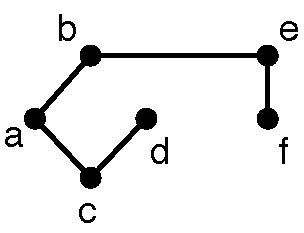
\includegraphics[width=2in]{min-spanning-tree/graph-pistol-st-1}
%
\hspace{1in}
%
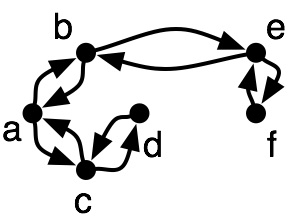
\includegraphics[width=2in]{min-spanning-tree/graph-pistol-st-1-traversal}
\end{center}
\end{example}

Now, recall that in the TSP problem it is assumed that there
is an edge between every pair of vertices.
\begin{question}
Can you find a way to derive a non-optimal solution to TSP using the
particular approach to visiting vertices?  Let's first try to
eliminate multiple visits.
\end{question}
Since it is possible to take an edge from any vertex to any other, we
can take shortcuts to avoid visiting vertices multiple times.  More
precisely what we can do is when about to go back to a vertex that the
tour has already visited, instead find the next vertex in the tour
that has not been visited and go directly to it.  We call this a
shortcut edge.

\begin{example}
The figure on the right shows a solution to TSP with shortcuts, drawn
in red.  Starting at $\vname{a}$, we can visit $\vname{a}, \vname{b}, \vname{e}, \vname{f}, \vname{c}, \vname{d}, \vname{a}$.

\begin{center}
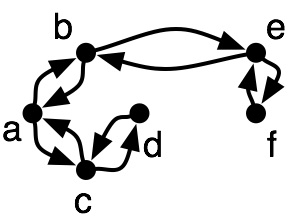
\includegraphics[width=2in]{min-spanning-tree/graph-pistol-st-1-traversal}
%
\hspace{1in}
%
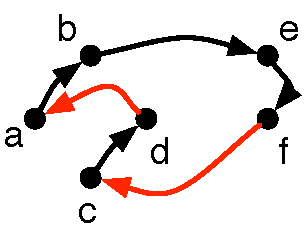
\includegraphics[width=2in]{min-spanning-tree/graph-pistol-st-1-traversal-once}
\end{center}

\end{example}

\begin{question}
Assuming that edges are distances between cities, can we say anything
about the lengths of the shortcut edges?
\end{question}

By the triangle inequality the shortcut edges are no longer
than the paths that they replace.  Thus by taking
shortcuts, the total distance is not increased.
\begin{question}
What can you say about the weight of the TSP that we obtain in this way? 
\end{question}
Since the Euler tour traverses each edge in the minimum spanning tree
twice (once in each direction), the total weight of the path is
exactly twice the weight of the MST.  With shortcuts, we obtain a
solution to the TSP problem that is at most the weight of the Euler
tour, and hence at most twice the weight of the MST.  Since the weight
of the MST is also a lower bound on the TSP, the solution we have
found is within a factor of 2 of optimal.  This means our approach is
an approximation algorithm for TSP that approximates the solution
within a factor of 2.   This can be summarized as:

\[W(\mbox{MST}(G)) \leq W(\mbox{TSP}(G)) \leq 2 W(\mbox{MST}(G))~.\]

\begin{remark}
It is possible to reduce the approximation factor to 1.5 using a well
known algorithm developed by Nicos Christofides at CMU in 1976.  The
algorithm is also based on the MST problem, but is followed by finding
a vertex matching on the vertices in the MST with odd-degree, adding
these to the tree, finding an Euler tour of the combined graph, and
again shortcutting.  Christofides algorithm was one of the first
approximation algorithms and it took over 40 years to improve on the
result, and only very slightly.
\end{remark}

\section{Problems}

\begin{probl}{}
There are 18 subgraphs for a triangle consisting of three vertices
and three edges connecting them, including the empty graph and the graph
itself.    List them all.
\end{probl}


\begin{probl}{}
In star contraction, what is the probability that a vertex with degree
$d$ is removed.
\end{probl}


\begin{probl}{}
Find an example graph, where star-based graph contraction removes a
small number of edges on each round.
\end{probl}

% Solution: a graph consisting of small stars that are connected with
% many edges. The star will be removed but all the cross edges between
% them will remain.  Must repeat this recursively to find the right
% structure.

\begin{probl}{}
Describe how to construct a graph that exhibits the worst-case
behavior for \thmref{gc::star-contraction-cost}.
\end{probl}

\begin{probl}{}
Is the star contraction algorithm work-optimal for a dense graph with
$\Omega(n^2)$ edges? Prove or disprove.
\end{probl}




\flushchapter
